%!TEX root = ../Thesis.tex
\chapter{Service Requirements for Aggregators} % (fold)
\label{cha:services}
\begin{marginfigure}
	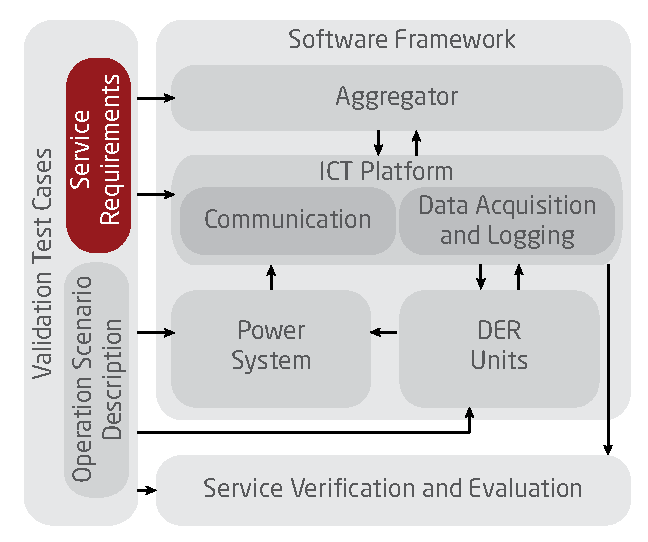
\includegraphics[width=\textwidth]{framework_services.eps}
	\caption{This chapter focuses on the \emph{service definition} block of the aggregator validation framework presented in Chapter~\ref{cha:validation}.}
      \label{fig:framework_services}
\end{marginfigure}
\newchapter{I}{t is clear from} Chapter~\ref{cha:validation} that \emph{service requirements} is an essential block in the aggregator validation framework (see Figure~\ref{fig:framework_services}). Initially, an objective of this work was to model service requirements in order to perform the aggregator validation. While this objective was achieved, it is clear that current service requirements in many countries are directly, or indirectly, blocking the integration of aggregators providing DR\fcite{cappers2013assessment,coalition2014mapping}. If aggregators are to be successfully integrated into the power system, the rules and requirements for participation must be changed. This chapter presents two novel contributions to integrating aggregators in the power system: a modeling method for services, and a proposal for the restructuring of requirements for ancillary services. A method for modeling services is important because the resulting models form the benchmark for the performance evaluation and verification of the aggregator (see Chapter~\ref{cha:verification}), as well as being a direct input to the aggregator (see Chapter~\ref{cha:aggregator}). The redefinition of ancillary service requirements is important since it will allow system operators to utilize the properties of all available resources, both traditional and new, in an optimal way.

The concepts presented in this section are part of two draft journal papers\fcite{bondy2016method,bondy2016redefining} which can be found in Appendix~\ref{app:segan} and Appendix~\todo{Berkeley Ref}, as well as work done as a collaborating author for a conference paper\fcite{heussen2013a} and a technical report written for the iPower consortium\fcite{bondy2014flech}.

%Content of this chapter is the work done at LBNL and through the iPower demo.
%\begin{itemize}
%	\item Service definition
%	\item What are aggregators expected to deliver?
%	\item PowerMax service requirements
%	\item Redefining Ancillary Services Requirements for Technology Agnostic Resources
%\end{itemize}

Aggregators/DR provide flexibility, as it is, they are not being paid for flexibility as defined previously, but only for power. This needs rethinking.\todo{fit this line somewhere, it is important!}
\section{Background}\label{sec:backgroundservices} % (fold)
\newsection{T}{he following section outlines} concepts related to the definition and requirements of services at TSO and DSO level. While services for the TSO (ancillary services) are well established, DSO services are a relatively new concept which has been explored in iPower project\fcite{ipower2013development}.
\subsection{What are Ancillary Services?} % (fold)
\label{sub:ancillaryservicesdef}
Defining what \gls{as} are, as well as which services the term includes, is difficult. This is due to both the differences in the way power systems are managed around the world and the differences in the terminology used to refer to such services. There is overlap between the European and US definition\fcite{eurelectric2004,ferc1997} of AS in that both describe them as services used to ensure the reliability of the power system. In both European and US context reliability is addressed by considering \emph{system adequacy} and \emph{security} \footnote{NERC also used the term system security, but in September 2001 security became synonymous with homeland protection in the US. Now it uses the term \emph{operating reliability} \cite{nerc2007definition}}. \emph{System adequacy} is the power system's ability to supply the electricity demand at all times and \emph{security} is the ability to withstand sudden disturbances.

Generally, maintaining an adequate and secure power system means maintaining the power system operating at nominal frequency and voltage. In cases where the power system deviates from nominal operation, either due to natural fluctuations in production/consumption or faults in the system, the system operators will activate ancillary services to restore normal operation. 

There exists a variety of ancillary services\todo{put a reference and examples}, but this work focuses on those that use active power to maintain the nominal frequency of the grid. In Europe\footnote{ENTSO-E recently changed its nomenclature of AS, and the three presented here correspond roughly to the classical primary, secondary and tertiary reserves as presented in \cite{Rebours}.} these services are \glspl{fcr}, \glspl{frr} (either automatic or manual), and \glspl{rr}\fcite{entsoe2013network}.
% subsection What are Ancillary Services? (end)
\subsection{Service Requirements for Ancillary Services} % (fold)
\label{sub:servreqAS}
Because AS are essential for the secure operation of the system, the system operators have requirements and restrictions on the units providing AS. A super-set of requirements across different systems is defined in \fcite{Rebours}. These requirements can roughly be classified into three categories:
\begin{description}
	\item[temporal requirements] which relate to how fast and for how long a service must be delivered;
	\item[resource tuning requirements] which relate to specific values that tuning parameters in the resource must have;
	\item[market requirements] which relate to bid sizes and similar parameters in systems where services are acquired through market mechanisms.
\end{description}

Of these three categories, only the temporal requirements relate to service performance. Furthermore, in most systems, the requirements are implicitly defined for traditional generation units. This means that most service requirements are oriented towards the least common denominator of service providers, e.g. a unit providing FCR should provide half of the service within 15 seconds and full response within 30 seconds\fcite{EnerginetAncillary}. A variety of generation and consumption units would be able to provide this service faster, but this quality is not rewarded. Another example is the requirement of having a PI-controller on units providing FRR in order to track the \gls{agc} signal. Such a controller is infeasible on distributed systems, but other modern controllers can provide offset-free control with similar properties. This means that the historical requirements for units participating in AS markets in many countries act implicitly, or explicitly, as barriers for new technologies to enter the market\fcite{cappers2013assessment,coalition2014mapping}.\todo{should I put in a more thorough description of FCR, FRR and RR, like what we have in the DDRAS paper?}

The concept of using demand side management to help the secure operation of the power grid has existed in different forms since the late 1970s\fcite{lampropoulos2013history}. But in recent years, the introduction of new consumption and generation technologies, \ie DERs, along with the roll-out of a smart metering infrastructure and the advances in ICT, has lead to the new opportunities in using smart control of small scale consumption/production as a service to the power grid. There is a large body of literature\fcite{oconnell2014benefits} concerning DR, and proposals to use it for AS\fcite{vrettos2015integrating,mathieu2012using,zarogiannis2014dynamic}.%\clearpage
% subsection Service Requirements for Ancillary Services (end)
\subsection{Distribution System Services} % (fold)
\label{sub:dsoservices}
As the amount of DERs installed at distribution level increases, the DSOs face new operational problems. Mainly, the increase in electric load will cause congestion and voltage issues. The traditional way of handling these are through reinforcement of the grid assets. Given the high cost of installing new cables, and the uncertainty in how the electricity consumption will change in the future, the use of flexibility services will be an attractive alternative.

One of the main outcomes of the iPower project was the definition of a set of flexibility services that demand aggregators can provide DSOs\fcite{ipower2013development} for congestion management or voltage issues. The requirements for three of the congestion management services have been further detailed individually\footnote{The services requirements were detailed in the following technical reports\cite{hansen2013flech,biegel2014flech,bondy2014flech}.}, and aggregator architectures have been designed to provide both congestion management\fcite{hu2014coordinated} and voltage support\fcite{han2014assessment}. At the same time, the concept of the \gls{flech} has been designed as a platform to enable the transparent contracting of flexibility\fcite{heussen2013a}.

% subsection DSO Services (end)
\subsection{Asset Management Services} % (fold)
\label{sub:assetmanagementservices}
In Chapter~\ref{cha:aggregator} the concept of \gls{ams} is introduced as the services that an aggregator provides to the owner of the DERs, or flexibility assets. An example of this is the case where the aggregator is an EV fleet operator that has the contractual responsibility of maintaining all EVs in the fleet within a certain \gls{soc}. The purpose of validating aggregators for these services is that flexibility asset owners can use the validation as a trust measure.

The main idea behind AMS is that the flexibility assets have a primary purpose, which is to satisfy the needs of their owner. The aggregator can use the flexibility of the units as long as the primary purpose is respected. Thus, from the perspective of customer comfort, an aggregator that is better at AMS is more desirable. 
% subsection Asset Management Servc (end)
% section Background on Aggregator Services (end)
\section{Modeling of Service Requirements} % (fold)
\label{sec:Modeling of Ancillary Services}
\newsection{T}{he validation framework} presented in Chapter~\ref{cha:validation} uses the \emph{service requirements} as a benchmark towards which the aggregator is evaluated. Currently, requirements for services are encoded within the contractual agreements between system operator and service provider. A method for translating the contracts into a model that the validation framework can use was developed.
The method consists of the following six steps:
%form have been identified as a generic method for modeling ancillary services. The steps are exemplified by DSO services defined in  and TSO services defined in :
\begin{enumerate}
  \item Identify physical parameters defining the service.
  \begin{itemize}
    \item \eg Power production or consumption, measured grid frequency, time measurements, etc.% Including maximum measuring sensitivities.
  \end{itemize}
  \item Identify the dynamic behaviors of the service related to system parameters (if any).
  \begin{itemize}
    \item \eg FCR expects a linear relation between a deviation from the nominal grid frequency and the generator set-point.% Power-cap has a dynamic relationship between feeder load and the controllable load power in order to keep the total feeder load at a $P_{DSO,Ref}$ value.
    %\item PowerMax is not dynamic. The aggregator must control $\Delta P_{Agg}$ to ensure that he does not violate $P_{max,Agg}$. But the service does not require a dynamic behavior related to a system parameter like primary frequency regulation and PowerCap.
  \end{itemize}
  \item Identify the physical size of the service and the tolerated error. % Both ideal service and minimum required service.
  \begin{itemize}
    \item \eg the volume of the bid for FCR. %Physical size is for example $P_{max,Agg}$ for PowerMax service or
%    \item Tolerance is for example $P_{max,Agg}+P_{tolerance}$ for the PowerMax service and allowed dead-band for DK1 primary reserve.
  \end{itemize}
  \item Identify the ideal response time of the service and acceptable response.
  \begin{itemize}
%    \item Most contracts comes with some timing specifying how fast the service provider must act.
    \item \eg FCR in western Denmark must be 50 \% of activated within 15 s and 100 \% within 30 s.
%    \item The ideal service is for example an instantaneous step in power to 100 \% of set-point for DK1 primary reserve.
  \end{itemize}
  \item Based on the dynamics, size and timing of the service, as well as the tolerated errors from points 1--4, develop a time series for ideal and acceptable service provision. The model will be a set of time series: $\mathbf{x}_{ideal}(t)$ for ideal response and $\mathbf{x}_{acc}(t)$ for acceptable response. Both time series can be a scalar or a vector, e.g. $\mathbf{x}_{acc}(t)$ can be formed by a set of upper and lower tolerance bounds or simply by an upper bound.
  \item Identify how the service error is to be measured.
\end{enumerate}

  %§$\mathbf{x}_{ideal}(t)$ and $\mathbf{x}_{acc}(t)$ can be a pair of values, e.g. minimum and maximum tolerance limits, for some services and may be only a single value, e.g. minimum or maximum tolerance, for others. 
From the frequency related AS and distribution level flexibility services described in Section~\ref{sec:backgroundservices} three kinds of services are identified:
\begin{description}
	\item[Reference Tracking:] Services where a reference signal must be followed, \eg regulation in the United States.
	\item[Band Service:] Services where 
	\item[Cap Service:]
\end{description}
% section Modeling of Ancillary Services (end)
%
\section{Redefining Ancillary Service Requirements} % (fold)
\label{sec:Redefining Ancillary Service Requirements}

% section Redefining Ancillary Service Requirements (end)
% chapter Service Requirements (end)

